\section{Method} \label{sec:method}

\begin{figure}[ht]
  \centering
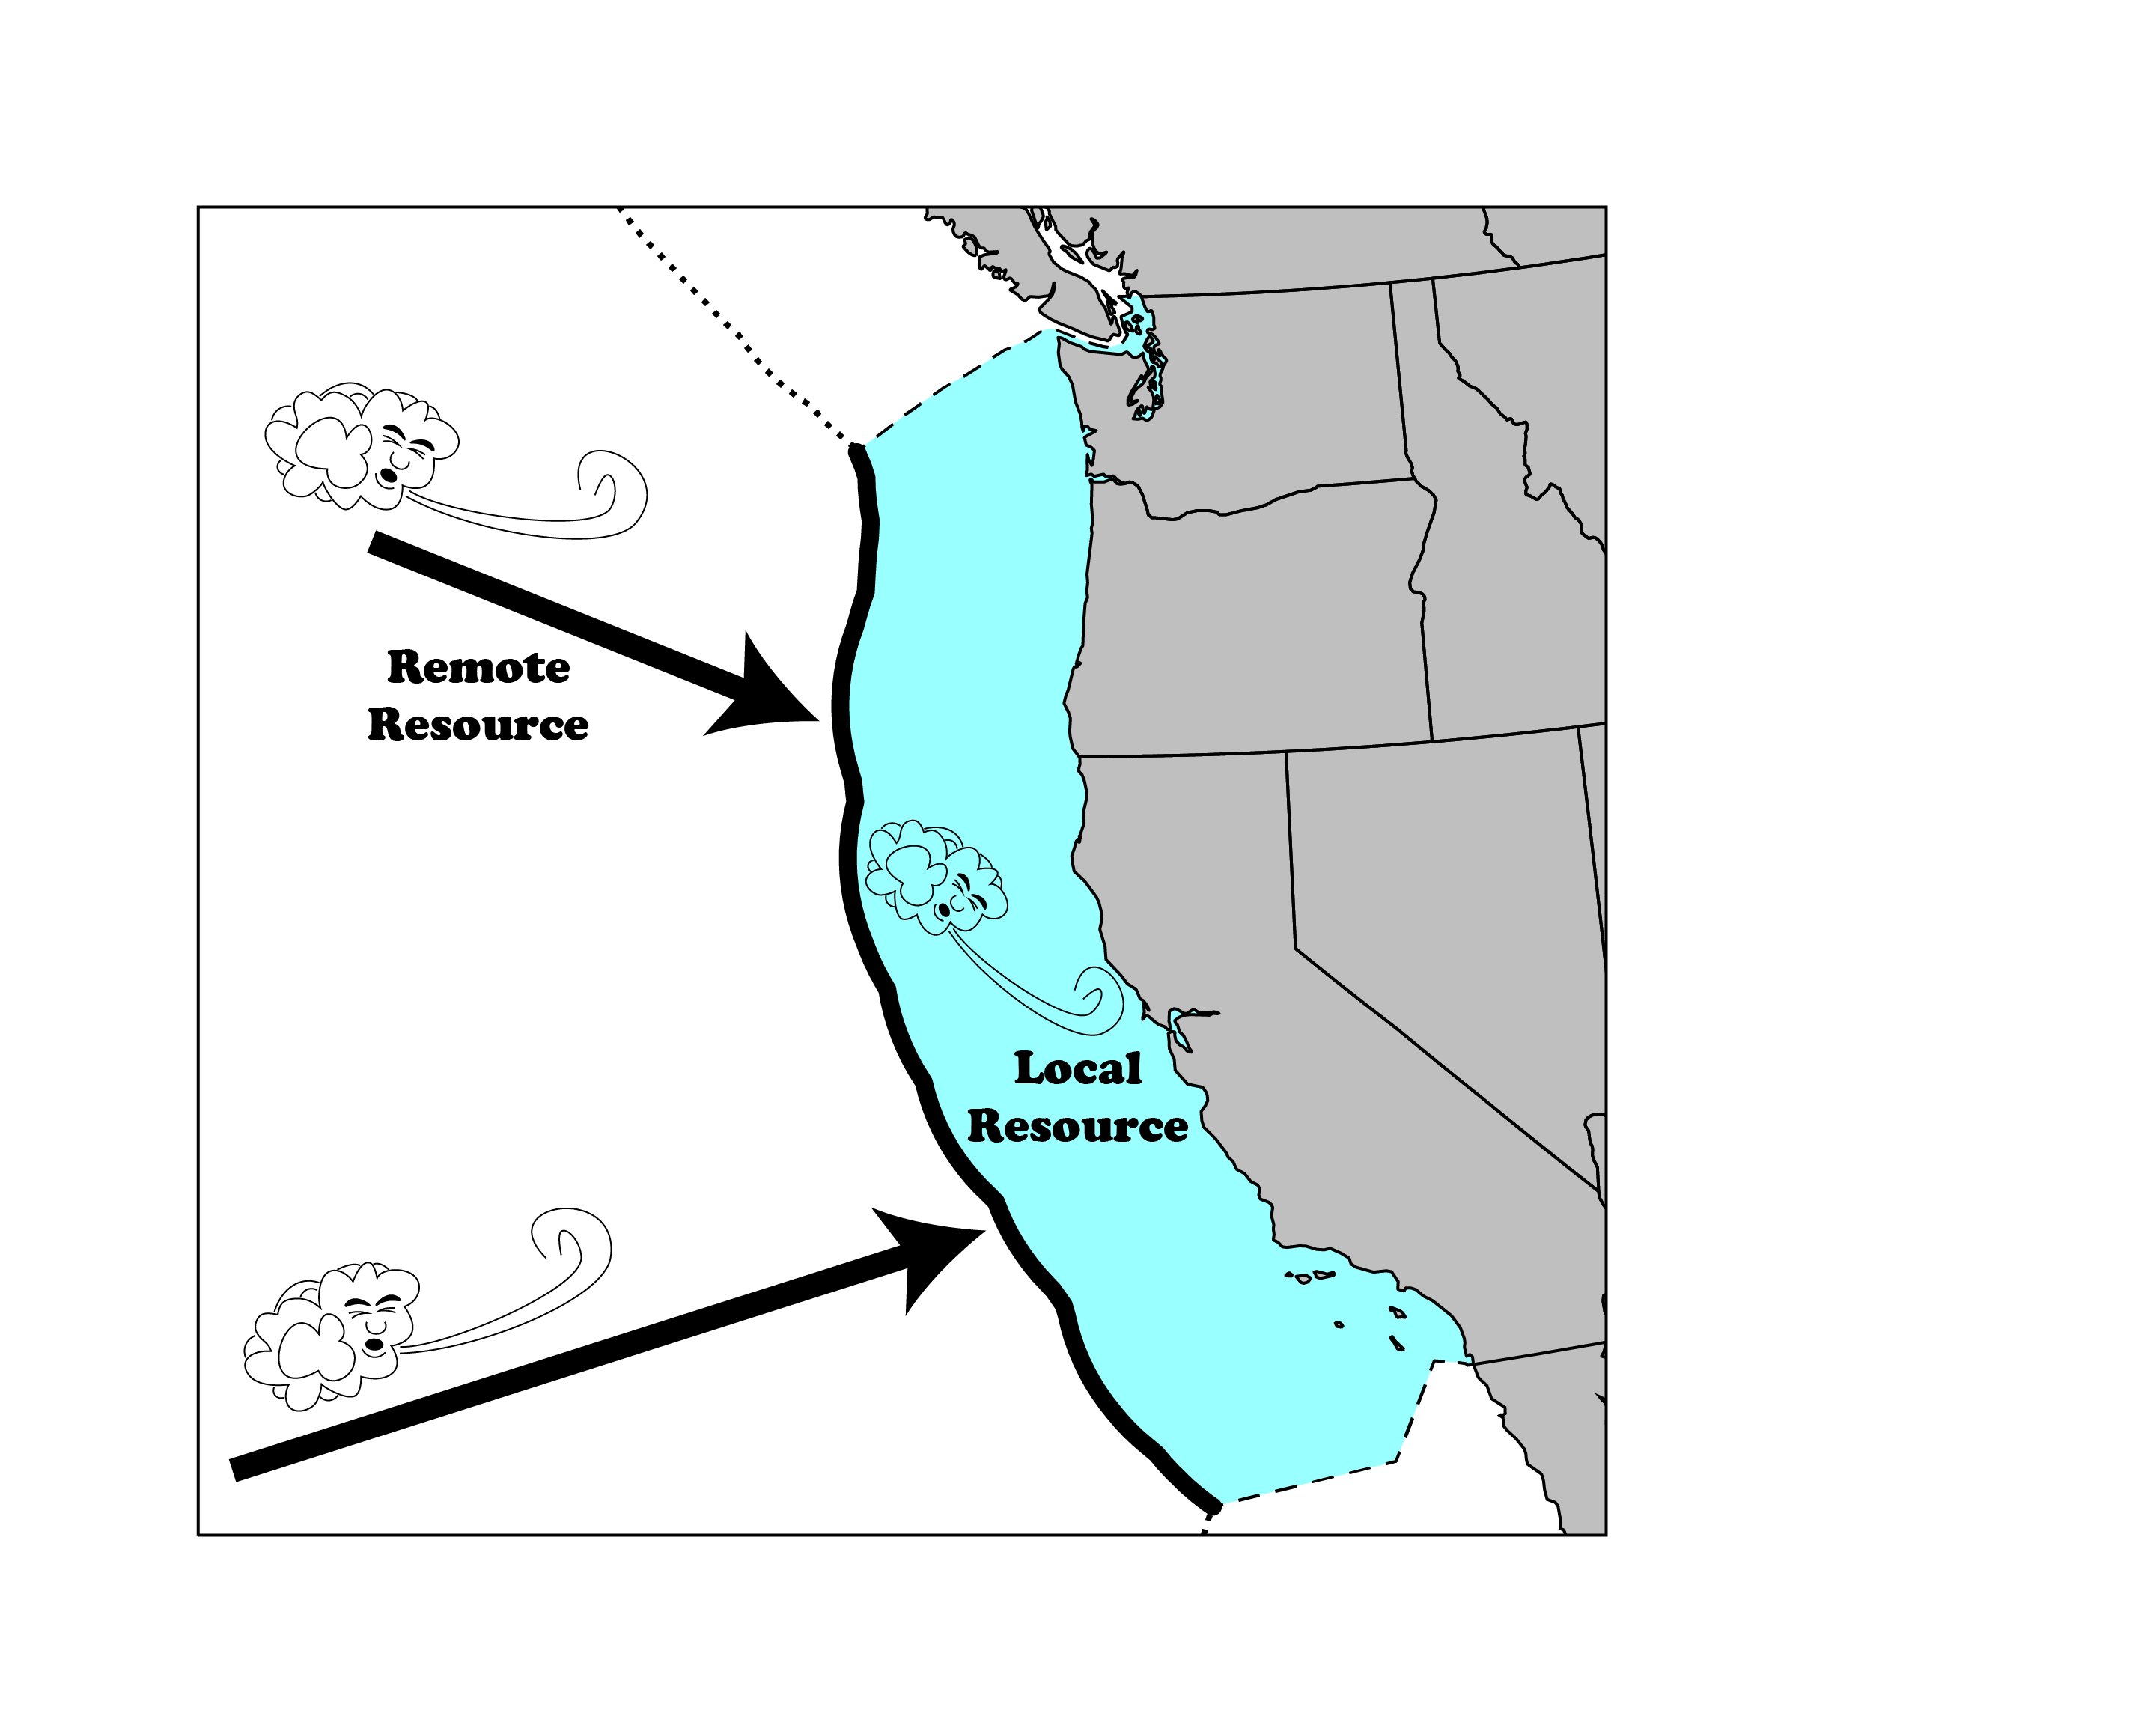
\includegraphics[width=0.9\linewidth]{../diagram/EEZ_contour03_edit01.png}
  \caption{A diagram depicting the U.S. West Coast’s ‘remote’ (arrows) and ‘local’ (cyan region) resource.}
  \label{fig:diagram:west-eez}
\end{figure}

The overarching goal of this study is to develop an accurate methodology for estimating the total theoretically available wave resource for a given region. The methodology has been formulated to address outstanding critiques of earlier works, namely: the method should eliminate or at least minimize ``double counting'', and it should also include all sources of wave energy that are legitimately a portion of the region's resource. With these objectives in mind, we propose that regional resource assessment should be conducted according to the following principles:

\begin{enumerate}
\item {\bf Follow IEC TS-101 standards for numerical model setup, configuration, and validation.} The IEC standards have done an excellent job of describing detailed guidelines for model setup and procedures for validation. We have followed the ``Class 1, Reconnassance" level here \note{RIGHT?!, or did we follow class 2?, ... or did we not follow IEC?!}, and it is most likely the most relevant class for other regional assessments, but there may be cases where it is desirable to follow class 2 or 3. One thing that should be added to the IEC guidance is the model must be configured to output the source terms, so that the `local resource' (below) can be computed.
\item {\bf The total resource is the sum of the remote and local resource} (Figure \ref{fig:diagram:west-eez}). The majority of existing wave resource assessments have considered the remote resource only. The inclusion of the local resource is a means for accounting for the 'recovery' of the wave-field downstream of where energy is extracted.
\begin{itemize}
    \item {\bf Calculate the ``remote resource'' utilizing a one-way dot-product at the boundary of the domain.} This approach has been used in several previous wave resource assessments \citep{gunnQuantifyingGlobalWave2012,hemerRevisedAssessmentAustralia2017}. This is a fundamental component of wave resource assessment because it avoids the {\em double} counting inherent in the `unit-circle' method used in EPRI 2011, and also avoids {\em under} counting that can occur when using a traditional dot-product. A detailed investigation of the importance of this approach can be found in Appendix \ref{appendix:one-way-method}.
    \item {\bf Include the local wave generation:} this consists of quantifying the wave resource generated landward of the boundary. Considering this part will provide a complete quantification of the resource. Estimates of the resource generated locally has implications to estimating the wave recovery potential, should a significant amount of wave energy be harvested. To the authors' knowledge this has not been considered in previous resource assessments.
\end{itemize}
\item {\bf Extend the assessment to the edge of the region's legal boundaries.} Based on Article 56 of the U.N. Law of the Sea — which states that "in the exclusive economic zone, the coastal State has sovereign rights [to] the production of energy from the water, currents and winds" — we propose that national resource assessments should utilize the EEZ as the domain over which wave energy resource totals are calculated \citep{unitednationsgeneralassemblyConventionLawSea1982}. Furthermore, the sum of the resource computed for two regions independently should be the same as if the resource is computed for both regions combined. In particular, this means that the method should not count wave energy fluxing across the boundary between the two regions.
\end{enumerate}

\subsection{Numerical Model} \label{sec:method:model}

Wave resource assessments typically rely on the use of wave model `hindcasts' to estimate the history of the wave field over the region(s) of interest, and then to compute estimates of the theoretical resource from the model output. The reason for this is that in-situ or remote measurements do not cover the oceans with enough resolution, spatially and temporally, to characterize the spatial variations of waves that occur at short scales. 
In this work all wave climate hindcasts are simulated using WAVEWATCH III\textregistered v5.16 \citep{tolmanDistributedmemoryConceptsWave2002,tolmanwavewatch}.

WAVEWATCH III\textregistered (hereafter WW3) is a  well established numerical model that has been implemented successfully in many previous wave resource assessments \citep[e.g.,][]{garcia-medinaWaveResourceAssessment2014,hemerRevisedAssessmentAustralia2017,yangWaveModelTest2017}.
WW3 solves the five-dimensional action balance equation:

\begin{align}
  \frac{d N}{d t} = \frac{\Src{tot}}{\sigma} = \frac{1}{\sigma}\left ( \Src{in} + \Src{ds} + \Src{brk} + \Src{nl} + \Src{bot} \right )
\end{align}
where $N(t,x,y,\sigma,\theta) \equiv D/\sigma$ is the wave action, $D$ is the variance spectrum, $t$ is time, $x$ and $y$ are the spatial coordinates, $\sigma$ is the radian frequency, and $\theta$ is the direction of wave propagation.
The wave action is conserved in the absence of sinks and sources of energy, their combined effect is represented as $\Src{tot}$.
The models do not include ocean currents so that $\sigma$ (intrinstic frequency) is spatially constant, and therefore wave energy (i.e., variance, $D$) is a conserved quantity (i.e., energy is only gained or lost by the source terms above).

In this study we implement the ``ST4'' physics package option in WW3 to simulate wind energy input ($\Src{in}$) and dissipation due to whitecapping ($\Src{ds}$) \citep{ardhuinObservationSwellDissipation2009}.
The wind forcing (for both the global and regional domains) is taken from NOAA's Climate Forecast System Reanalysis (CFSR) \citep{sahaNCEPClimateForecast2010}. The non-linear quadruplet interactions ($\Src{nl}$) are modeled with the Hasselmann and Hasselmann (\citeyear{hasselmannComputationsParameterizationsNonlinear1985}) formulation. Bottom friction ($\Src{bot}$) and depth induced wave breaking ($\Src{brk}$) are modeled with the JONSWAP Hasselmann etal. \citeyear{hasselmannMeasurementsWindwaveGrowth1973} and Battjes and Janssen \citeyear{battjesEnergyLossSetup1978} models, respectively. Finally, the effect of sea ice is considered by using a time varying mask based on the ice coverage fields from CFSR. Default parameters are used for all formulations.

\note{Someone (Hagermann?) told me that: ST4 gives improvement in power density and Hs, but overpredicts energy-period. Is this true? Citation?}\textcolor{green}{I did some searching and didnt find a good discussion about this.} \note{Should we just drop this detail then? Or ask Hagermann?}


The WW3 simulations span a 32-year period from January 1, 1979 to December 31, 2010. The first year (1979) is treated as a 'spin-up' year, and is not included in any calculations of resource totals. Variability in the wave climate on timescales longer than the 31-year period included in the average are not considered (i.e., changes in the wave resource due to climate change are not included). The wave spectrum is discretized with 24 equally spaced bins in $\theta$ space and 29 logarithmically spaced frequency bins from 0.035Hz to 0.5Hz with an increment factor of 1.1. 

Model grids and bathymetry come from the NOAA NCEP hindcast Phase 1 mosaic-model \citep{chawla2011wavewatch,chawla201230}. In this system a global model (0.5$^{\circ}$ resolution) drives regional models (10" - 4" resolution) providing complete coverage over the U.S. EEZ with higher resolution focused on shallower waters. This model was reimplemented to store wave spectra and source terms at a high resolution.

Model output is collected at the U.S. EEZ around Alaska (excluding the Arctic Coast), Atlantic Coast, Caribbean Coast (Puerto Rico and U.S. Virgin Islands), Gulf Coast, Hawaii (excluding the Papah$\bar{\text{a}}$naumoku$\bar{\text{a}}$kea Marine National Monument), and the West Coast. Full variance spectra are stored at the U.S. EEZ boundary (at 200 nmi from shore, and along EEZ `borders' with other nation's). Inside the EEZ, directionally integrated source term output is collected at lines of equal distance from shore from 18.5 km (10 nmi) to 351.9 km (190 nmi) every 18.5 kms. Both output types are collected at hourly intervals every 1/6$^{\circ}$ along the defined lines.

This model configuration is mostly aligned with the IEC TS 62600-101 requirements for a reconnaissance class resource assessment. The requirements for physical processes are met with the exception of the inclusion of wave-current interactions and the effect of tides. It is not expected that the tides will influence waves significantly beyond 18.5 km from shore. Wave-current interactions can be important particularly around the Gulf Stream, thus the exclusion of this must be revisited in future studies. The numerical requirements from IEC TS 62600-101 indicate that spherical coordinates must be used with a minimum temporal resolution of 3h, 25 wave frequency components, 24 azimuthal directions, and a minimum spatial resolution of 5 km. All but the latter are met in this study, the regional models at 4" have a meridional resolution of 7.4 km.

In WW3, as it is customary in third-generation spectral wave models, the waves are computed over a specified spectral width after which a spectral tail is appended to represent the energy in the high frequencies \citep[e.g.][]{ardhuinObservationSwellDissipation2009}. This frequency cutoff is generally the minimum of the highest described frequency and the cutoff supported by the source term formulations. The simulations in this study are performed with the default high frequency cutoff:

\begin{align}
  f_{c} = \frac{2.5}{T_{m01}}
\end{align}
where $T_{m01}$ is the mean spectral period. The source term integrals are performed for the range where the wave spectrum is actively simulated.

\subsection{Calculate Resource Totals} \label{sec:method:calc}

In this work we propose that the total theoretical wave resource, $R_T$, be defined as a sum of `remote' and `local' components:
\begin{align}
  R_T = R_R + R_L
\end{align}
The remote resource, $R_R$, is the piece of the wave energy resource that has previously been defined as the total wave resource \citep{gunnQuantifyingGlobalWave2012,EPRIwaveresource2011}, while the local resource, $R_L$, has not previously been included in wave resource assessments.

\subsubsection{Remote Resource} \label{sec:method:calc:remote}

The remote resource is computed as a line-integral of the wave energy that fluxes toward the coastline across the EEZ boundary when it is bordered by international waters. 

\begin{align}
  R_R = \rho g \int_{\ell}\iint \delta \, c_g(f) \, \bar{D}(f,\theta) \d f \d \theta \d l
\label{eqn:RR}
\end{align}
Where $c_g(f)$ is the wave group velocity, $\ell$ is the integration contour, and $\delta$ is the directionality coefficient which we take to be $\delta = \cos(\theta_n - \theta)$ for waves propagating toward the coastline, and $\delta = 0$ otherwise. $\theta_n$ is the direction of the normal to the integration contour pointing toward the coastline. The `one-way' condition ensures that waves propagating offshore are not {\em subtracted} from the total \citep[]{gunnQuantifyingGlobalWave2012}. A detailed rationalle for the one-way approach to estimating $R_R$ is included in appendix \ref{appendix:one-way-method}. The over-bar denotes a time-average of the wave-variance spectrum over the 31-year period from Jan. 1 1980, through Dec 31, 2010.

In this work, the integration contour $\ell$ is the segments of the U.S. EEZ that separate U.S. EEZ waters from the open-ocean (hereafter the `EEZ boundary'; thick black line in Figure \ref{fig:diagram:west-eez}), and does not include the EEZ segments that separate one nation's EEZ from that of a neighbor (hereafter the `EEZ borders'; thin dashed lines) \citep[]{flandersmarineinstituteMaritimeBoundariesGeodatabase2018}. This is because wave-energy that fluxes across EEZ borders will be counted -- using the methodology described here -- by the nation from which that resource originated. For example, waves that propagate southward across the Canada-U.S. EEZ border are counted as Canada's resource, and waves that propagate northward across this border are counted as U.S. resource. Either way, these waves will already have been counted in the originating nation's resource, and so including wave fluxes across these borders would only lead to `double counting'.


\subsubsection{Local Resource} \label{sec:method:calc:local}

While neglecting the local resource may be reasonable for small projects, the fact that it
typically has been implicitly ignored has raised legitimate questions about the validity of the methodologies, which has led to skepticism and confusion. The local resource is computed as an area-integral of all wave source- and sink-terms, except for bottom friction:

\begin{align}
  R_L &= \rho g \int_{EEZ}\iint \left ( \bar{S}_{in} + \bar{S}_{ds} + \bar{S}_{brk} + \bar{S}_{nl} \right ) \d f \d \theta \d A
\label{eqn:RL}
\end{align}
where $dA$ is differential-area integral of the source terms. Since the model results are output in spherical coordinate system, the coordinates were transformed using an Albers equal area projection before performing the area integral. By performing these projections on a region-by-region basis with carefully chosen projection parameters, this approach introduces $<1\% $ local distortion at the edges of the largest regions (Alaska), and therefore introduces a $\ll 1\%$ error in the total estimate of $R_L$.

It should be noted that the terms $\bar{S}_{ds}$ and $\bar{S}_{brk}$ are both negative. The non-linear term ($\bar{S}_{nl}$) -- which serves primarily to redistributes energy from high to low frequency -- is also negative on average as there is a loss of energy in this transfer of energy.
Based on these facts, it is tempting to assume that wave energy originating from the large positive term $S_{in}$ could be absorbed prior to these other terms dissipating it because this approach would yield a significantly larger local resource.

While that approach would yield a significantly larger local resource, doing so is scientifically questionable for several reasons. First, the spatial and temporal scales at which $S_{in}$ delivers energy to the wave field is similar to the scales at which $S_{brk}$ \note{???(and $S_{ds}$)???} removes it. In other words, significant wave-breaking \note{and dissipation} occurs when winds generate waves. Second, the details of wave-generation is an active area of research, with large uncertainty associated with each term's magnitude \citep[e.g.,][]{garcia-medinaWaveResourceAssessment2014}. The sum of the terms, on the other hand, is relatively well constrained as demonstrated by the performance of wave models in general (i.e., via wave-model validation studies \note{NEED CITATIONS}). Third, there are significant practical questions about extracting small-wave energy (i.e., at the scales that the majority of $S_{in}$ energy exists) across sufficiently large spatial-area for the energy to be sizable.

There is certainly an inherent tension here between, ``including the local resource in order to provide a complete assessment of the {\em theoretical} wave resource'', and assuming that some pieces of the wave source terms (wind input) are inaccessible on {\em practical} and {\em technical} feasibility grounds. In other words, some might argue that including the negative source terms belongs in a technical or practical resource assessment. However, we argue that including $R_L$ as defined here is already a highly optimistic consideration.
The task of quantifying any resource, including the theoretical resource, involves making some assumptions about what is realistic and what is not. 
Perhaps more importantly, until we have a better understanding of the magnitude (i.e., uncertainty) of the individual terms, and we have technologies that show promise for extracting high-frequency energy at scales between wind-input and dissipation/breaking, neglecting those terms seems scientifically dubious.

The bottom-friction term, on the other hand, {\em is neglected} in this analysis primarily because those terms represent the ultimate destruction of wave energy at the coastlines. The objective of wave resource assessment is to quantify the wave energy available before it reaches this demise. 
\note{Is the above statement correct? In other words: is bottom-friction how energy is destroyed in the model, or is there a wave-breaking term? Or some other mechanism?}
% IS THERE MORE TO SAY HERE ALONG THE LINES OF:
% If these terms were included the local resource would be negative because all energy that enters or is created in the domain would be dissipated? \citep{garcia2013inner}

This piece has not typically been considered in wave resource assessments. This is most likely because it is obvious that for projects within 10 to 20 miles of shore - where it seems reasonable to assume the majority of projects will be for the next several decades - $R_L \ll R_R$. However, when we are taking the perspective of an assessment of the nation's resource - which according to the U.N. law of the sea legally extends to the edge of the U.S. EEZ - $R_L$ is an important piece of the total energy available. By accounting for this term, this methodology directly incorporates the energy added to the wave field over that area. While it does not directly address the question ``how quickly will the wave-field re-energize down-wave from a wave farm?'' It does explicitly include this energy. \note{Still not happy with this paragraph. What am I trying to say here?}

However, because the source terms in \eqref{eqn:RL} depend on the sea-state and the sea-state depends on energy extracted ``up-wave'', there is ambiguity in estimating $R_L$ related to where and when wave energy is extracted by WECs. To address this, we calculate two estimates of $R_L$. The first, `natural local resource' ($R_{L_\circ}$) is calculated from the source-terms where waves from the global domain propagate freely throughout the regional domain (the EEZ). The second, `potential local resource' ($R_{L_*}$) is calculated from the source-terms when no wave energy propagates across the EEZ boundary. In other words, this is a `lake case' that only contains waves generated by winds within the regional domain.

In all cases we examined, $R_{L_*}$ was found to be greater than $R_{L_\circ}$ (see Appendix \ref{appendix:flux-vs-area} for details). In the sense that $R_L$ is meant to be an estimate of the maximum energy available, this suggests that $R_L$ could be defined as being equal to $R_{L_*}$. However, the scenario of removing all wave energy from the wave field at the edge of the EEZ is so hypothetical that it seems unrealistic to use this value to define $R_L$. Therefore, we choose to treat these two estimates of $R_L$ as an uncertainty range for the value.

It is worth noting that -- though a line-integral that accounts for directionality of the wave flux (a {\em vector quantity}) is applicable for estimating $R_R$ \eqref{eqn:RR} -- directionality is {\em not } important to estimating $R_L$ correctly in \eqref{eqn:RL} (i.e., all directions are weighted equally). This is because the source terms are {\em scalar quantities} that are functions of direction per unit-area, and therefore an area-integral applies.
%This can be understood by considering the hypothetical case of an array of WECs that covers the entire EEZ. The wave energy that is added locally within the EEZ will be absorbed -- regardless of it's direction -- by the array before it reaches the edge of the EEZ where a line-integral would be appropriate (i.e., when directionality is important).


\subsection{Methodological differences with EPRI 2011}
\label{sec:method:changes}

Before proceeding to the results, we take a moment to briefly describe four major methodological differences between this work and EPRI 2011. First, we have utilized updated models \note{GGM: can you describe briefly the major changes here? Probably just a sentence or two?} Second, we utilize a one-way dot-product, where EPRI 2011 used the ``unit-circle'' method which the National Academy noted would cause double-counting. Third, we include the local resource, $R_L$, in the total. Finally, we extend the analysis to the edge of the EEZ (200 nautical miles from shore), where EPRI 2011 nominally used the 200 meter isobath, or a 50 nautical miles from shore line, depending on the region.

%%% Local Variables:
%%% TeX-master: "wave_res"
%%% End:
